\chapter{Εισαγωγή τεχνολογίας του Κυβερνήτη(\en{Kubernetes})}

\section{Εισαγωγή-Η λογική της λειτουργίας του Κυβερνήτη}

Τα τελευταία χρόνια, παρατηρείται ραγδαία αύξηση στον τομέα της πληροφορικής, 
με την εμφάνιση και εξάπλωση νέων εννοιών, όπως ο κυβερνήτης και τα \en{microservices}. 
Ένας βασικός παράγοντας που συνέβαλε στην εισαγωγή αυτών των τεχνολογιών είναι η ικανότητα εικονικοποίησης 
του λειτουργικού συστήματος, καθώς και η δυνατότητα εκτέλεσης εφαρμογών ως κοντέινερ. 
Αυτές οι τεχνολογίες επιτρέπουν την απομόνωση και τη διαχείριση εφαρμογών με μεγαλύτερη ευελιξία και 
αποτελεσματικότητα, κάτι που έχει οδηγήσει σε σημαντικές αλλαγές στον τρόπο ανάπτυξης και λειτουργίας των σύγχρονων υποδομών λογισμικού

Τα κοντέινερ είναι ένας καλός τρόπος για να ομαδοποιήσουμε και να εκτελέσουμε τις εφαρμογές μας. 
Σε ένα περιβάλλον παραγωγής, πρέπει να διαχειριστούμε τα κοντέινερ που εκτελούν τις εφαρμογές και να 
διασφαλίσουμε ότι δεν υπάρχει χρόνος διακοπής λειτουργίας. Για παράδειγμα, εάν ένα κοντέινερ πέσει κάτω, ένα άλλο κοντέινερ πρέπει να ξεκινήσει. 

Έτσι έρχεται να σώσει την κατάσταση ο κυβερνήτης. Το \en{Kubernetes} σάς παρέχει ένα πλαίσιο για να εκτελείτε τα κατανεμημένα συστήματα με ευελιξία. 
Φροντίζει για την κλιμάκωση και το \en{failover} για την εφαρμογή σας, παρέχει μοτίβα ανάπτυξης και πολλά άλλα. Δε θα αναλύσουμε με κάθε λεπτομέρεια
τι ακριβώς είναι ο κυβερνήτης γιατί μία τέτοια προσπάθεια είναι μία διπλωματική από μόνη της αλλά θα προσπαθήσουμε να παρουσιάσουμε τα βασικά χαρακτηριστικά τα οποία
χρησιμοποιήθηκαν πρακτικά στη διπλωματική.

\section{Το αποθετήριο κοντεινερ-\en{Docker Desktop}}

Προκειμένου να μπορέσουμε να χρησιμοποιήσουμε το \en{Docker Desktop} θα πρέπει να έχουμε φτιάξει την εφαρμογή μας σαν κοντεινερ.

Για να γίνει αυτό θα πρέπει να φτιάξουμε το παρακάτω \en{Dockerfile} το οποίο ουσιαστικά είναι η εφαρμογή μας αλλά σε κοντεινερ.

\begin{figure}[htb]
	\centering
	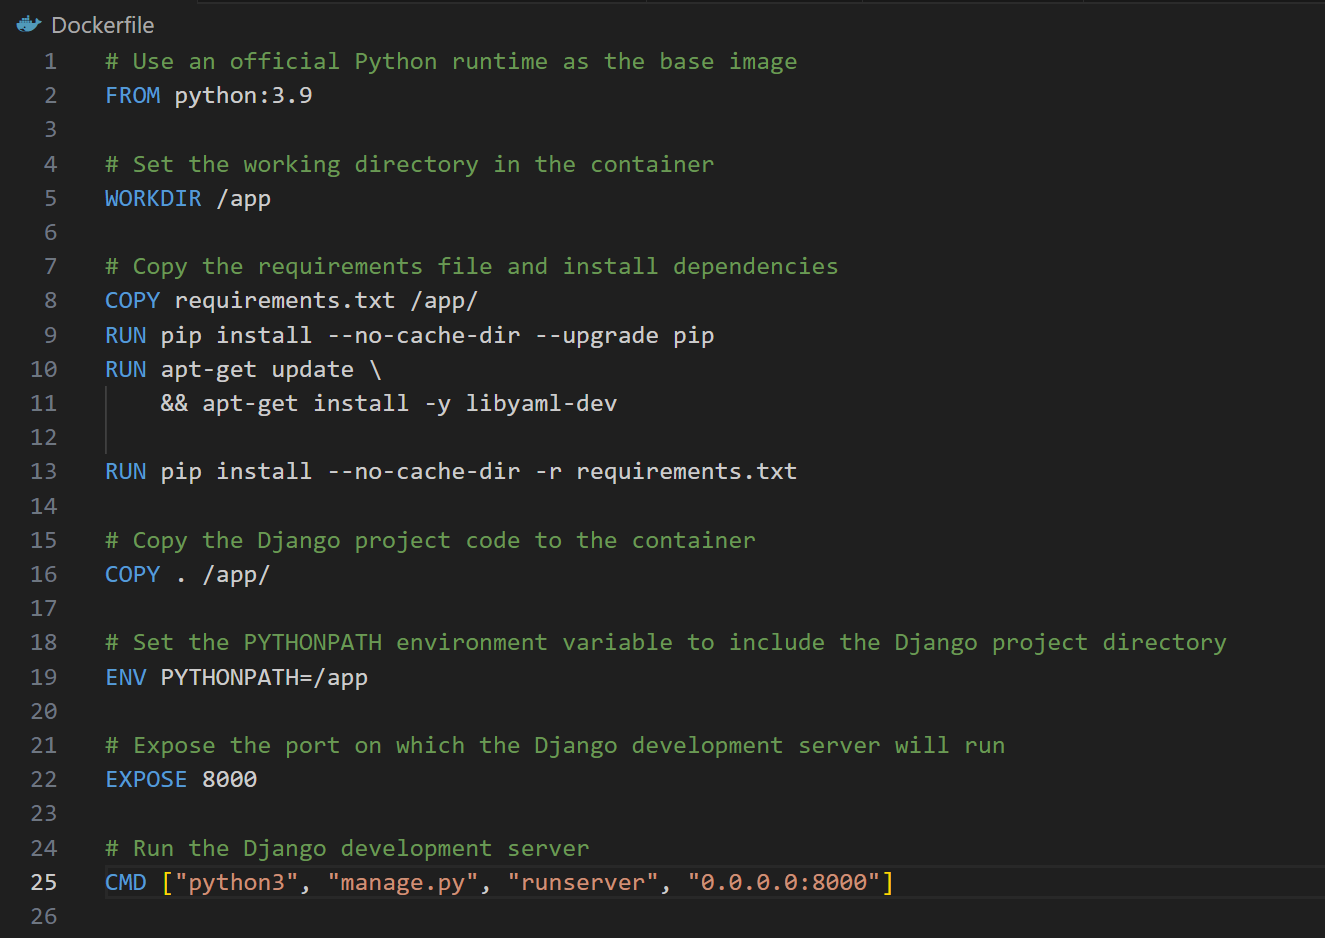
\includegraphics[width=1.5\textwidth]{graphics/dockerfile.png}
	\caption{\en{Dockerfile}}
\end{figure}

\FloatBarrier


Για να φτιάξουμε το \en{image} τρέχουμε τη παρακατω εντολη

\FloatBarrier
\begin{figure}[h]
	\centering
	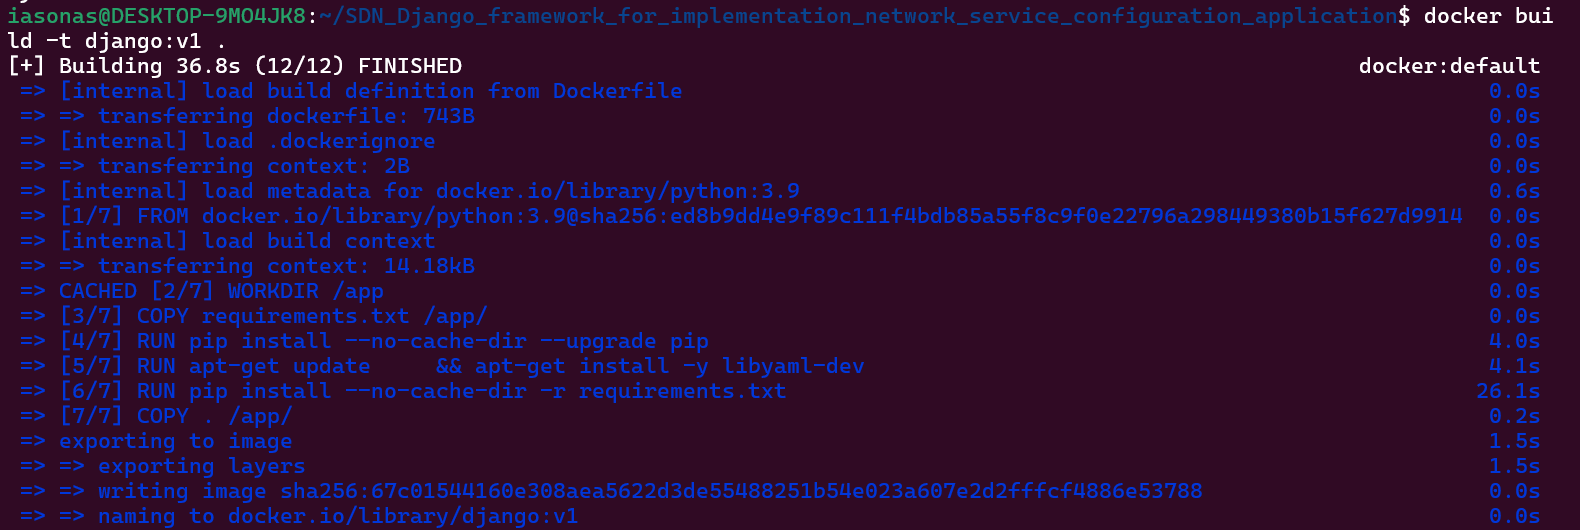
\includegraphics[width=1.5\textwidth]{graphics/docker_build.png}
	\caption{\en{Docker build}-Δημιουργία του κοντεινερ}
\end{figure}


Θα πρέπει μετά να βάλουμε το \en{image} στο \en{DockerDesktop} και αφού γίνει αυτό θα μπορέσουμε να την τρέξουμε στην υποδομή του κυβερνήτη.
Το ίδιο μπορεί να γίνει και χωρίς την εφαρμογή \en{DockerDesktop} αλλά τρέχοντας το \en{Docker service}
απευθείας πάνω στο \en{WSL2} όπως φαίνεται και στις παρακάτω εικόνες.

\FloatBarrier
\begin{figure}[h]
	\centering
	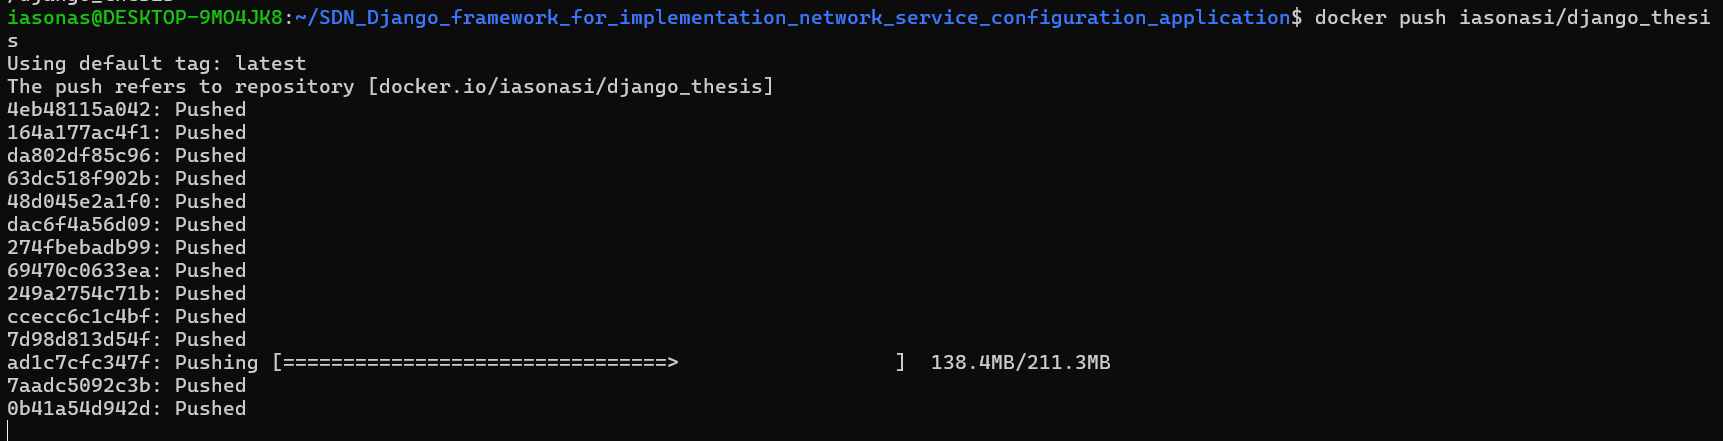
\includegraphics[width=1.5\textwidth]{graphics/dockerpush.png}
	\caption{\en{Docker push}-}
\end{figure}

\begin{figure}[h]
	\centering
	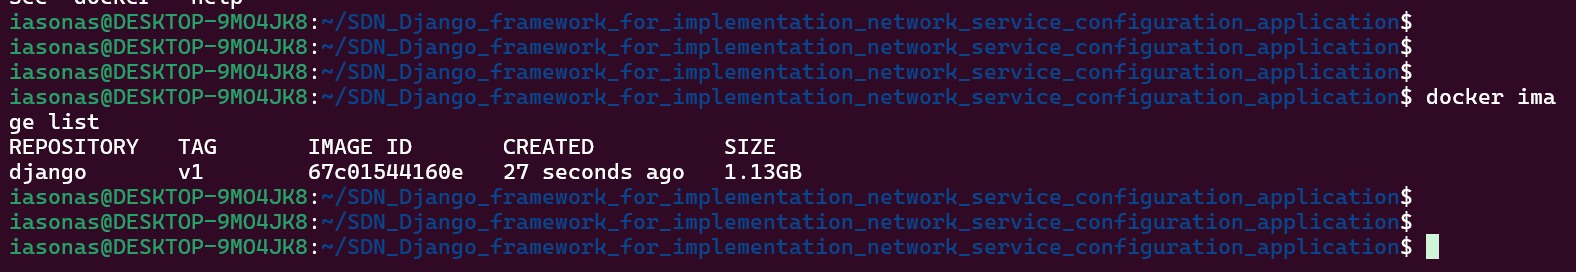
\includegraphics[width=1.5\textwidth]{graphics/docker_image_list.png}
	\caption{\en{Docker image list}}
\end{figure}


\section{Κυβερνήτης}

Στη διπλωματική αυτή εργασία, χρησιμοποιείται ένα τοπικό περιβάλλον 
ανάπτυξης με \en{Kubernetes} μέσω του \en{Minikube} και του \en{WSL2}
(\en{Windows Subsystem for Linux} 2) για την ανάπτυξη και δοκιμή 
της εφαρμογής \en{Django}. 

Το \en{Kubernetes} είναι μια δημοφιλής 
πλατφόρμα ενορχήστρωσης κοντέινερ, που επιτρέπει την αυτόματη 
διαχείριση και κλιμάκωση εφαρμογών σε περιβάλλοντα παραγωγής, 
ενώ το \en{Minikube} προσφέρει τη δυνατότητα εκκίνησης ενός 
τοπικού \en{Kubernetes cluster}. 
Με τον τρόπο αυτό, επιτυγχάνεται η δημιουργία ενός ασφαλούς, 
απομονωμένου περιβάλλοντος δοκιμών, το οποίο προσομοιώνει ένα 
πλήρες \en{cluster}, χωρίς την ανάγκη πρόσθετης υποδομής \en{cloud}.

Χάρη στο \en{WSL2}, το οποίο επιτρέπει την εκτέλεση \en{Linux} 
πυρήνα απευθείας στα \en{Windows}, 
εξασφαλίζεται ευκολία στη διαχείριση του \en{cluster} 
και της εφαρμογής \en{Django}, 
ενώ η χρήση εργαλείων όπως το \en{kubectl} 
καθιστά εύκολη την παρακολούθηση και τον έλεγχο των \en{pods} 
και υπηρεσιών. Αυτό το περιβάλλον προσφέρει μια ολοκληρωμένη 
εμπειρία ανάπτυξης και δοκιμής, βοηθώντας στην κατανόηση των 
αρχών του \en{Kubernetes} και διευκολύνοντας τη μετάβαση της 
εφαρμογής σε μεγαλύτερα \en{production} περιβάλλοντα

Το \en{Minikube} είναι ένα εργαλείο που απλοποιεί την εκτέλεση και 
διαχείριση ενός τοπικού \en{Kubernetes cluster} στον υπολογιστή σας,
ειδικά σχεδιασμένο για περιβάλλοντα ανάπτυξης και δοκιμών. 
Σας επιτρέπει να ξεκινήσετε ένα \en{Kubernetes cluster} 
με ένα μόνο κόμβο (ή ακόμα και πολλούς σε ορισμένες περιπτώσεις) 
χρησιμοποιώντας εικονικοποίηση μέσω \en{WSL, Docker, ή Hypervisor}. 
Ο κύριος σκοπός του \en{Minikube} είναι να παρέχει ένα περιβάλλον \en{Kubernetes} 
με όλες τις βασικές δυνατότητες του \en{Kubernetes} 
αλλά χωρίς την πολυπλοκότητα που θα απαιτούσε η διαχείριση ενός \en{cluster}
σε παραγωγικό περιβάλλον.

Επιπλέον, το \en{Minikube} 
διαθέτει ενσωματωμένα εργαλεία, όπως τη δυνατότητα να παρακολουθείτε
και να διαχειρίζεστε τον πίνακα ελέγχου του \en{Kubernetes}, 
να δημιουργείτε \en{pods, deployments}, και \en{services}, και 
να παρακολουθείτε τα \en{logs} των εφαρμογών σας, ενώ επιτρέπει 
επίσης εύκολη σύνδεση με εργαλεία όπως το \en{kubectl} 
για πλήρη πρόσβαση στη διαχείριση του \en{cluster}. 
Αυτό το καθιστά ιδανικό για προγραμματιστές που θέλουν να 
πειραματιστούν με \en{Kubernetes}, 
να κάνουν δοκιμές εφαρμογών, ή να αναπτύξουν μικροϋπηρεσίες 
τοπικά χωρίς να απαιτείται η πολυπλοκότητα ενός πλήρους \en{cluster}
όπως το περιβάλλον της παρούσας διπλωματικής εργασίας. Παρακάτω μπορούμε να δούμε 
πόσο εύκολα μπορούμε να ξεκινήσουμε ένα τοπικό περιβάλλον κυβερνήτη.


\begin{figure}[h]
	\centering
	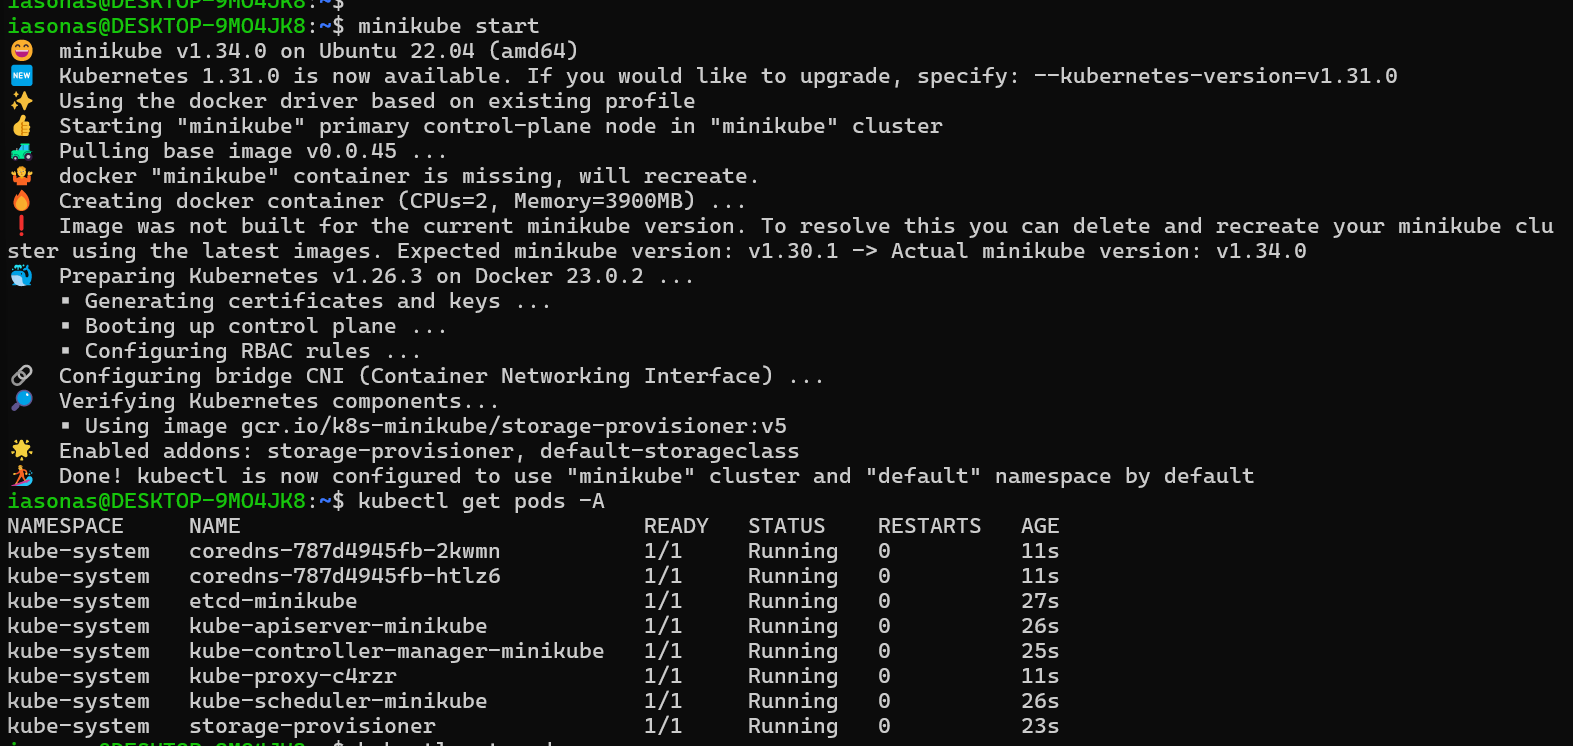
\includegraphics[width=1.5\textwidth]{graphics/minikube_deployment_k8s.png}
	\caption{\en{Minikube deployment}}
\end{figure}


Στο πλαίσιο της ανάπτυξης της εφαρμογής, χρησιμοποιήθηκε το 
\en{Kubernetes} για τη δημιουργία και διαχείριση ενός \en{pod} 
που φιλοξενεί την εφαρμογή \en{Django}. Το αρχείο διαμόρφωσης \en{YAML}
(\en{pod1.yml}) που δημιουργήθηκε, ακολουθεί τη βασική δομή του \en{Kubernetes}, 
ορίζοντας τον τύπο πόρου ως \en{Pod} και 
εκχωρώντας μεταδεδομένα όπως το όνομα \en{djangotestapp}. 
Στην ενότητα \en{spec}, ορίζεται ένα \en{container} 
το οποίο χρησιμοποιεί την εικόνα \en{iasonasi/djangotestapp:latest} 
και ακούει στη θύρα 8000, η οποία είναι η προεπιλεγμένη θύρα της 
εφαρμογής \en{Django}.

Αυτό το παράδειγμα αποδεικνύει τη σημασία της χρήσης του \en{Kubernetes YAML syntax} 
για την αυτοματοποιημένη ανάπτυξη και διαχείριση \en{containerized} 
εφαρμογών. Μέσω αυτής της διαδικασίας, η εφαρμογή μπορεί να 
επεκταθεί εύκολα σε διάφορα περιβάλλοντα και να κλιμακωθεί 
ανάλογα με τις ανάγκες. Το συγκεκριμένο αρχείο \en{YAML} 
επιτρέπει στο \en{Kubernetes} να εκτελέσει και να διαχειριστεί το 
\en{pod} με τρόπο ανεξάρτητο από το υποκείμενο σύστημα, 
εξασφαλίζοντας επαναληψιμότητα και δυνατότητα μεταφοράς του 
συστήματος σε διαφορετικές υποδομές. Στην παρακάτω εικόνα φαίνεται το 
\en{YAML file} που χρησιμοποιήθηκε. Φυσικά ολόκληρος ο κώδικας βρίσκεται
ανοιχτός και προσβάσιμος στο \en{GITHUB}


\begin{figure}[h]
	\centering
	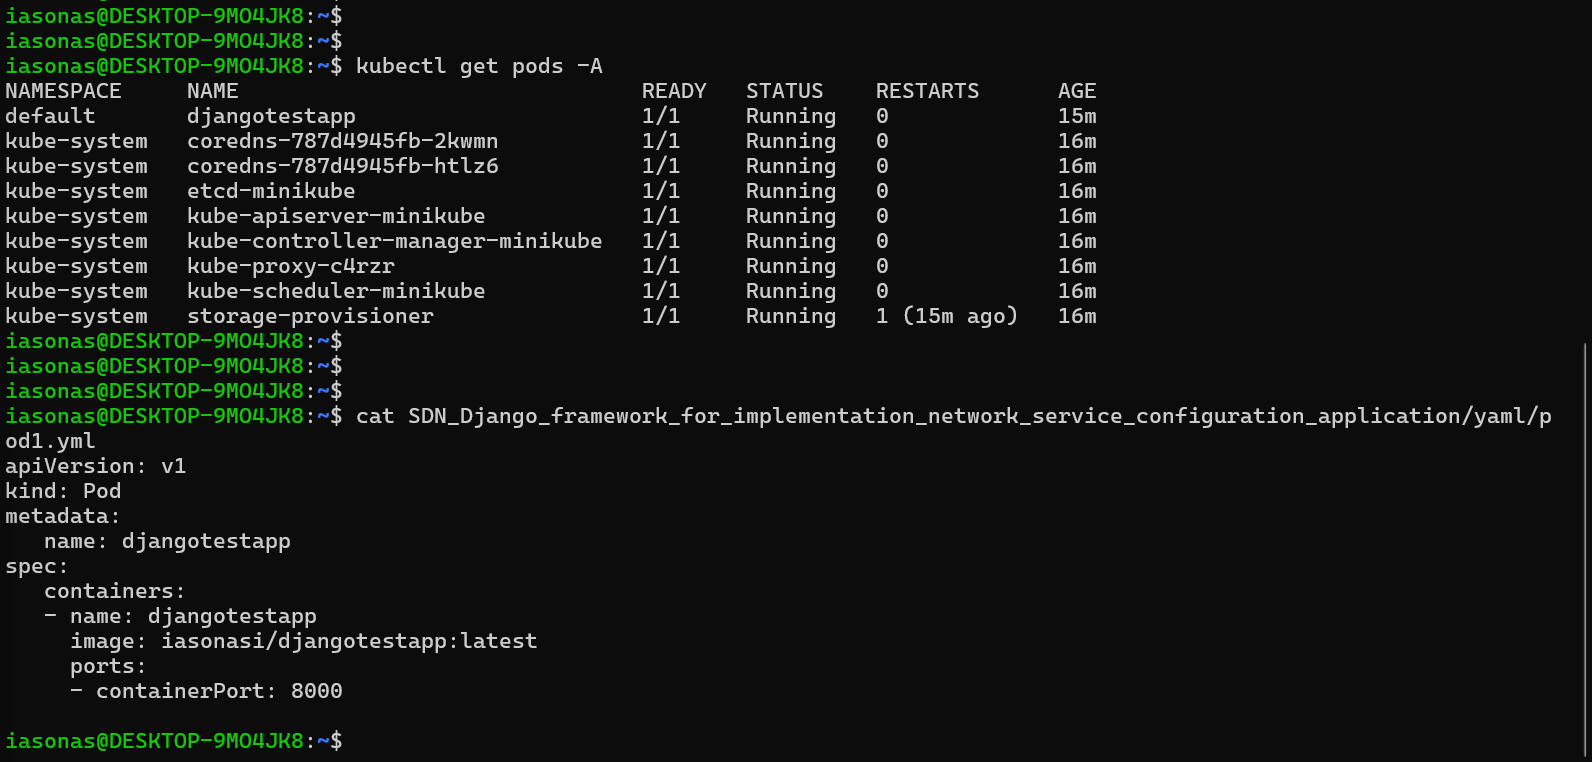
\includegraphics[width=1.5\textwidth]{graphics/deploy_django.png}
	\caption{\en{Django Deploy}}
\end{figure}

